\documentclass{article}
\usepackage[utf8]{inputenc}
%allow simultaneous greek and english input
\usepackage[greek,english]{babel}
\usepackage{alphabeta}
%package needed for image template
\usepackage{eso-pic}
%colour links, hrefs, etc whatever colour you like
%use only if needed. Shows warnings on Greek characters but nothing bad actually happens.
%just annoys you

%\usepackage[colorlinks = true,
            %linkcolor = black,
            %urlcolor  = black,
            %citecolor = blue,
            %anchorcolor = blue]{hyperref}

%Change default LaTeX contents name and figure name to Greek
\addto\captionsenglish{
    \renewcommand{\contentsname}{Περιεχόμενα}
    \renewcommand{\figurename}{Εικόνα}}
    %create a macro named BackgroundPic for setting a background on the first page
\newcommand\BackgroundPic{
    \put(-3,0){
    \parbox[b][\paperheight]{\paperwidth}{%
    \vfill
    \centering
    
\includegraphics[width=\paperwidth,height=\paperheight]{LATEX_TEMPLATE_V2.pdf}
    \vfill
    }}}
%Info
\title{\vspace{0.2cm}\textbf{Μια εισαγωγή στο Quadrature Amplitude Modulation (QAM)}}
\date{\textbf{Μάιος 2021\\ Έκδοση 1.1\\[8pt] Ασύρματα Συστήματα και Δίκτυα}}
    \author{\textbf{Μπαντής Αστέριος}}
%include page geometry packages
\usepackage{natbib}
\usepackage{amsmath}
\usepackage{graphicx}
\usepackage[a4paper, total={6.5in, 8in}]{geometry}
%document starts here, who would have imagined that?
\begin{document}
%set LATEX_TEMPLATE_V2 as template JUST for this page
%the asterisk means it will be set just for this page
\AddToShipoutPicture*{\BackgroundPic}
 \maketitle
\maketitle
%leave a bunch of empty space for the contents. Change cm if needed.
\vspace{4cm}
%shows contents automatically. Every section, subsection, etc automatically shows up here
\tableofcontents{}
%change page
\pagebreak
%create new command about pics on all other pages
\ClearShipoutPicture
\newcommand\Bgpic{
    \put(-4,0){
    \parbox[b][\paperheight]{\paperwidth}{%
    \vfill
    \centering
    
\includegraphics[width=\paperwidth,height=\paperheight]{LATEX_TEMPLATE_V2.pdf}
    \vfill
    }}}
%set background picture for EVERY page after page 2, including page 2
%see, no asterisk
\AddToShipoutPicture{\Bgpic}
%yay, our first section, who would have thought

\section{Εισαγωγή}
\large
Πριν εξετάσουμε το Quadrature Amplitude Modulation, ας υπενθυμίσουμε κάποιες σημαντικές ιδιότητες. Όπως γνωρίζουμε, οι τρεις βασικές ιδιότητες μιας αναλογικής κυματομορφής είναι το πλάτος, η συχνότητα, και η φάση της. Ας πάρουμε σαν παράδειγμα ένα ημίτονο. Σύμφωνα με τις τρεις παραπάνω ιδιότητες, το σήμα αυτό μπορεί να μοντελοποιηθεί μαθηματικά ως εξής:
\Large
$$\mathrm{f(t)}=\mathrm{A}\cos(\mathrm{ωt+φ})$$
\large
Όπου, Α είναι το πλάτος, ω είναι η συχνότητα σε rad/s, και φ είναι η φάση σε rad. Αυτή η ιδιότητα μπορεί, φυσικά, να επεκταθεί και σε άλλα περιοδικά σήματα σύμφωνα με τη σειρά Fourier του κάθε σήματος. Χρησιμοποιώντας τουλάχιστον μία από τις ιδιότητες αυτές, είναι δυνατή η κωδικοποίηση ψηφιακής πληροφορίας πάνω σε ένα αναλογικό σήμα. Για παράδειγμα, το πλάτος του σήματος μπορεί να κωδικοποιηθεί έτσι ώστε η παρουσία σήματος ή το πλάτος $A_{1}$ να δίνει λογικό αληθές (1), ενώ η απουσία σήματος ή το πλάτος $A_{2}$ να δίνει λογικό ψευδές. Αντίστοιχα, η συχνότητα $ω_{1}$ μπορεί να κωδικοποιηθεί ως λογικό αληθές, και η συχνότητα $ω_{2}$ σαν λογικό ψευδές, ή η φάση $φ_{1}$ μπορεί να κωδικοποιηθεί ως "1" και η φάση $φ_{2}$ σαν "0".[1]\\
\begin{center}
    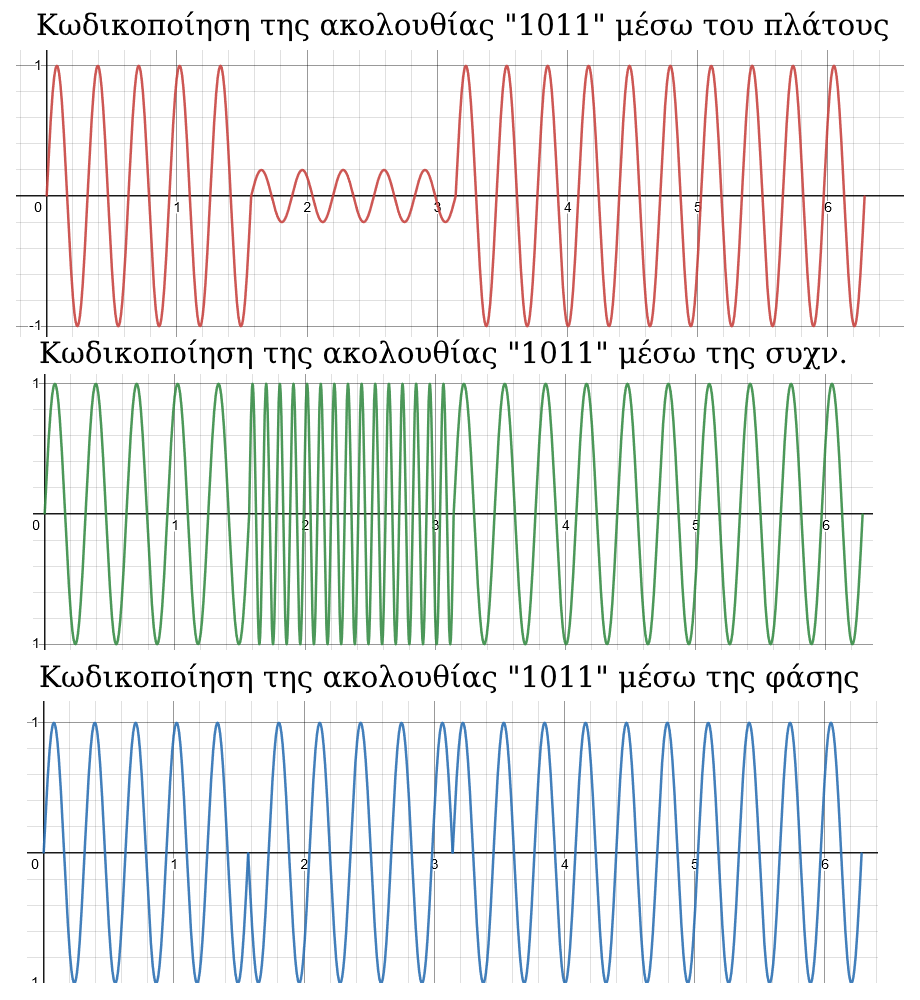
\includegraphics[scale=0.4]{diktya_pic1.png}
\end{center}
Το Quadrature Amplitude Modulation (QAM) είναι μια από τις σύγχρονες τεχνικές ψηφιακής κωδικοποίησης δεδομένων σε αναλογικό σήμα. Χρησιμοποιεί δύο εκ των τριών βασικών ιδιοτήτων που αναφέρθηκαν στις προηγούμενες παραγράφους: το πλάτος (Amplitude-Shift Keying) και τη φάση (Phase-Shift Keying). Ο σκοπός του QAM είναι η κωδικοποίηση πολλών bits μέσα στο ίδιο σύμβολο.[1]

\section{Μηχανισμός Λειτουργίας}
Για να καταφέρει το σύστημα να κωδικοποιήσει πάνω από ένα bit στο ίδιο σύμβολο, είναι αναγκαίος ο ορισμός κάποιων καταστάσεων λειτουργίας. Συγκεκριμένα, για $2^{n}$ συνολικό αριθμό καταστάσεων είναι δυνατή η κωδικοποίηση $n$ bits ανά σύμβολο. Οι καταστάσεις αυτές κωδικοποιούνται στο πεδίο Q-I, δηλαδή σε ένα καρτεσιανό σύστημα το οποίο απεικονίζει το σήμα σωστής φάσης (I, In-Phase) και το σήμα με φάση μετατοπισμένη κατά 90 μοίρες (Q, Quadrature).[1][2] Ας ρίξουμε μια ματιά στο κύκλωμα του πομπού, όπως έχει σχεδιαστεί στην πηγή 2, για έναν εκπομπό 16 καταστάσεων:
\begin{center}
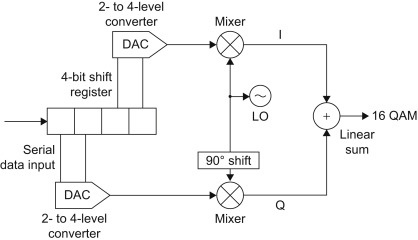
\includegraphics[scale=1.1]{diktya_pic2_right.jpg}
\end{center}
Με παρόμοιο τρόπο μπορεί να παραμετροποιηθεί για περισσότερα ή λιγότερα bits ανά σύμβολο, δηλαδή περισσότερες ή λιγότερες καταστάσεις. Το σκεπτικό παραμένει ίδιο. Παρατηρούμε πως ο πομπός του QAM μοιάζει αρκετά με τον πομπό του BPSK και του QPSK. Λογικό, αφού οι δύο αυτές καταστάσεις μπορούν να θεωρηθούν, υπό όρους, ειδικές περιπτώσεις του QAM. Ας εξετάσουμε το σύστημα Q-I. Έστω πως έχει 2 σημεία, άρα είναι VPSK (Binary PSK). Η απόσταση του σημείου από κέντρο των αξόνων θα δείχνει το πλάτος του σήματος εξόδου για το σύμβολο που αναπαριστά το σημείο, ενώ η γωνία του από το θετικό μέρος του άξονα I θα δείχνει τη φάση του σήματος εξόδου για το σύμβολο που αναπαριστά το σημείο. Το BPSK θα μπορούσε να ονομαστεί λανθασμένα και "2-QAM". Προφανώς, όμως, δεν έχουμε καταφέρει κάτι ακόμα, αφού κάθε σύμβολο αναπαριστά μονάχα ένα bit.[1][2]
\begin{center}
    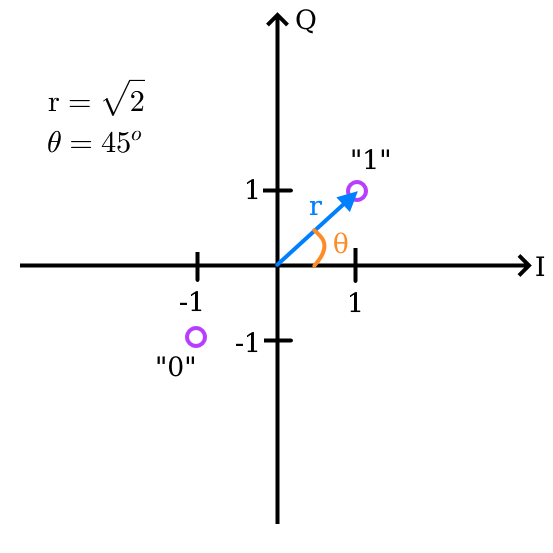
\includegraphics[scale=0.6]{diktya_pic3.png}
\end{center}
Ας δούμε τώρα τι γίνεται στην περίπτωση των τεσσάρων σημείων, δηλαδή εάν είχαμε κάτι που θα το "βαφτίζαμε" λανθασμένα 4-QAM.
Παρατηρούμε πως πλέον ένα σύμβολο αναπαριστά 2 bits. Όμως, ακόμα δεν έχουμε κάποια αλλαγή στο πλάτος. Η περίπτωση αυτή ονομάζεται QPSK (Quadrature PSK).[1]
\begin{center}
    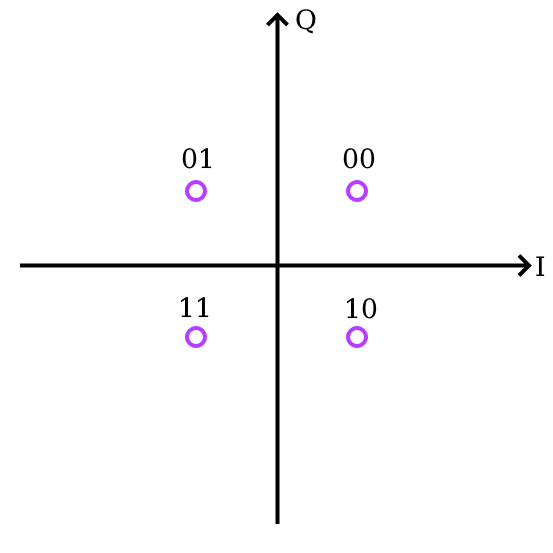
\includegraphics[scale=0.6]{diktya_pic4.png}
\end{center}
Για να κρατήσουμε τη συμμετρία, ας δούμε τώρα την περίπτωση των 16 σημείων, δηλαδή 16-QAM, και ένα σύστημα 64 σημείων, δηλαδή 64-WAM. Οι περιπτώσεις αυτές όντως ένα πραγματικό σύστημα QAM, αφού διαμορφώνουν το σήμα \emph{και} κατά πλάτος \emph{και} κατά φάση. Στα παραδείγματα αυτά χρησιμοποιείται ο κώδικας Gray για την "ονοματοδοσία" του κάθε σημείου.[3] Σημειώνεται πως η εικόνα του 64-QAM ανήκει στην έρευνα της πηγής 3.
\begin{center}
    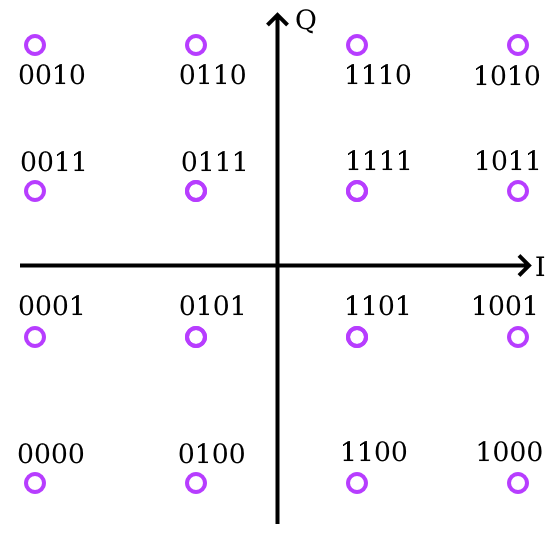
\includegraphics[scale=0.5]{diktya_pic5.png}\\
    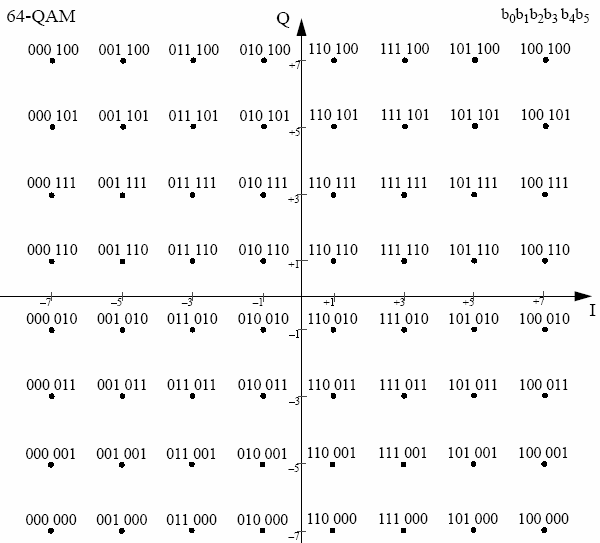
\includegraphics[scale=0.4]{64-QAM-Signal-Constellation-with-Gray-Coding.png}
\end{center}
Υπάρχουν αντίστοιχα περιπτώσεις 256-QAM, 1024-QAM, 4096-QAM κ.τ.λ. Αυτή η δυνατότη- τα αλλαγής του αριθμού των μέγιστων πιθανών καταστάσεων στη βιβλιογραφία συχνά ονομάζεται M-ary QAM, ή, ελληνιστί, μ-αδική τετραγωνισμένη διαμόρφωση πλάτους, όπου, φυσικά, το Μ αντιπροσωπεύει τον αριθμό καταστάσεων.\\[12pt]
Σε έναν ιδανικό κόσμο, προφανώς το σύστημα με περισσότερα bits ανά σύμβολο θα ήταν το καλύτερο, χωρίς μειονεκτήματα. Παρ' όλα αυτά, το δικό μας σύμπαν δε λειτουργεί έτσι. Λόγω του θορύβου, δεν υπάρχει εγγύηση πως το σήμα που θα στείλει ο πομπός μας θα είναι ακριβώς στο σημείο που είναι σχεδιασμένο στο διάγραμμα του αστερισμού QAM που έχουμε σχεδιάσει. Κατά συνέπεια, θα πρέπει, σε κάθε αστερισμό QAM, να δίνουμε και κάποιο περιθώριο. Είναι προφανές πως, για ένα ορισμένο bandwidth, θα έχουμε λιγότερα λάθη (και, συνεπώς, μεγαλύτερο περιθώριο για θόρυβο) όταν έχουμε λιγότερες καταστάσεις στον αστερισμό, δηλαδή λιγότερα bits ανά σύμβολο. Τα περιθώρια αυτά πρέπει να οριστούν έτσι ώστε να μην επικαλύπτεται κανένα με οποιοδήποτε άλλο, αλλά έτσι ώστε να μεγιστοποιήσει το περιθώριο, δηλαδή να ελαχιστοποιήσει τα λανθασμένα ή/και χαμένα σύμβολα. Οπότε, αναγκαστικά, μεγαλύτερο πλήθος καταστάσεων στον αστερισμό QAM χρειάζεται και μεγαλύτερο Signal to Noise Ratio (SNR). Για παράδειγμα στο πρωτόκολλο IEEE 802.11ac, για ένα κανάλι των 20MHz το ελάχιστο SNR για σύστημα QPSK είναι 5dB, για 16-QAM είναι 11dB, και για 64-QAM είναι 18dB.[1][4] 
\begin{center}
    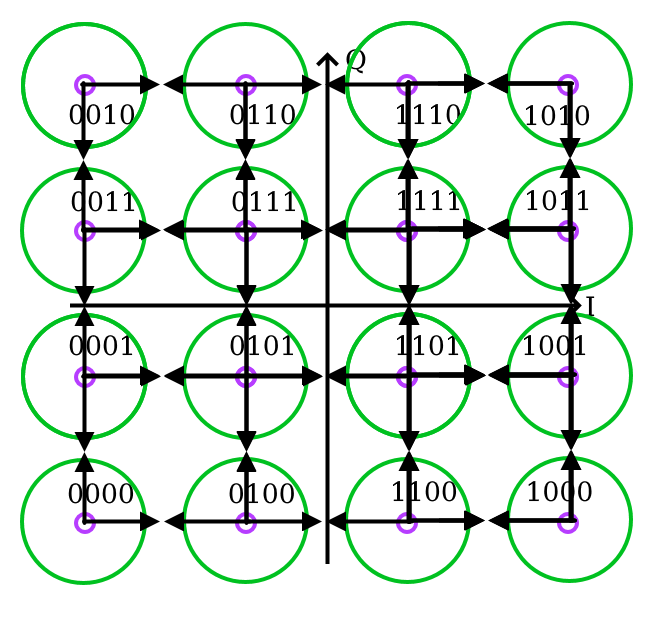
\includegraphics[scale=0.5]{diktya_pic6.png}
\end{center}
Σε αυτό το σημείο αξίζει να σημειωθεί πως δεν είναι απαραίτητο τα σημεία ενός αστερισμού QAM να είναι τοποθετημένα σε ένα ορθογώνιο. Ο αστερισμός αυτός μπορεί να είναι και μη-ορθογώνιος, δηλαδή να έχει κάποιο άλλο σχήμα. Οι μη-ορθογώνιοι αστερισμοί QAM εν γένει έχουν μεγαλύτερα περιθώρια θορύβου, άρα και λιγότερα λανθασμένα bits, όμως είναι αρκετά δυσκολότεροι στην κατασκευή τους.[5] Μπορούμε να δούμε ένα παράδειγμα στην παρακάτω εικόνα, η οποία ανήκει στις διαφάνειες της πηγής 5:
\begin{center}
    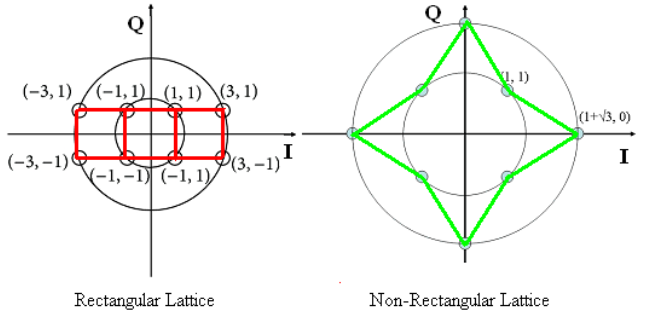
\includegraphics[scale=0.6]{image.png}
\end{center}
Ας δούμε, λοιπόν, πως θα έμοιαζε η ακολουθία "1011 1111 0101 0010" στο σύστημα 16-QAM που σχεδιάστηκε σε προηγούμενη εικόνα. Παρατηρούμε πως έχουμε καταφέρει να αποστείλουμε 4 φορές περισσότερα bits στο ίδιο χρονικό διάστημα.
\begin{center}
    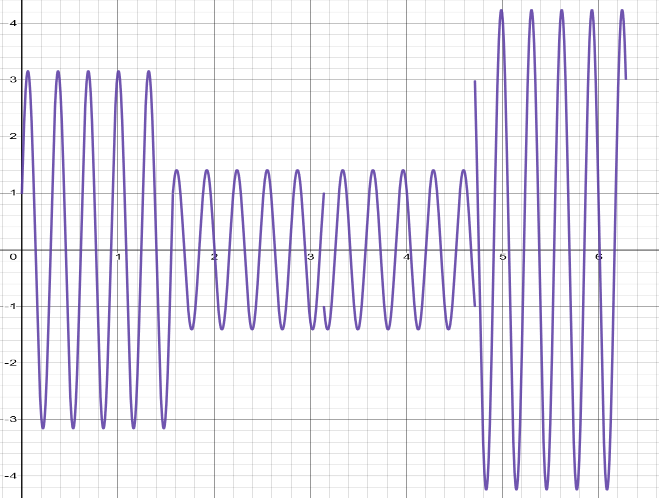
\includegraphics[scale=0.7]{diktya_pic7.png}
\end{center}
\section{Εξισώσεις}
Η καθαρά αλγεβρική μοντελοποίηση του QAM είναι η εξής:
$${\displaystyle s_{c}(t) = \cos(ω_{c}t)I(t)+{\cos \left(ω_{c}t+{\tfrac {\pi }{2}}\right)}\;Q(t)}$$
Οπότε αρκεί ένας πομπός να κάνει την αντίστροφη διαδικασία ως εξής:
$${\displaystyle r(t)=s_{c}(t)\cos(ω_{c}t)=I(t)\cos(ω_{c}t)\cos(ω_{c}t)-Q(t)\sin(ω_{c}t)\cos(ω_{c}t)}$$
Άρα έχουμε:
$${\displaystyle r(t)={\tfrac {1}{2}}I(t)\left[1+\cos(2ω_{c}t)\right]-{\tfrac {1}{2}}Q(t)\sin(2ω_{c}t)}$$
$$r(t)={\tfrac {1}{2}}I(t)+{\tfrac {1}{2}}\left[I(t)\cos(2ω_{c}t)-Q(t)\sin(2ω_{c}t)\right]$$\\[8pt]
Άρα αρκεί να χρησιμοποιήσουμε ένα χαμηλοπερατό φίλτρο (LPF) για το I(t), και να πολλαπλασιάσουμε ένα αντίγραφο του σήματος με ένα ημίτονο και έπειτα να χρησιμοποιήσουμε το LPF για το Q(t), για να αφαιρέσουμε την φέρουσα συχνότητα $ω_{c}$ και να παραλάβουμε το αρχικό σήμα. Ο μετασχηματισμός Fourier του σήματος είναι:
$${\displaystyle s_{c}(t)_{+}={\tfrac {1}{2}}e^{i2\pi ω_{c}t}[I(t)+iQ(t)]\quad {\stackrel {\mathcal {F}}{\Longrightarrow }}\quad {\tfrac {1}{2}}\left[{\widehat {I\ }}(ω-ω_{c})+e^{i\pi /2}{\widehat {Q}}(ω-ω_{c})\right]}$$
Παρατηρούμε ομοιότητες με τη διαμόρφωση πλάτους με διπλή πλαϊνή ζώνη και κατεσταλμένη φέρουσα (DSB-SC AM), κάτι απόλυτα λογικό. Ας δούμε κάποια παραδείγματα, ξεκινώντας με ένα σήμα AM DSB-SC[6] (Πηγή εικόνας: Σημειώσεις "Σήματα Πληροφορία και Επικοινωνία, Παπαδοπούλου Φωτεινή, 2020")
\begin{center}
    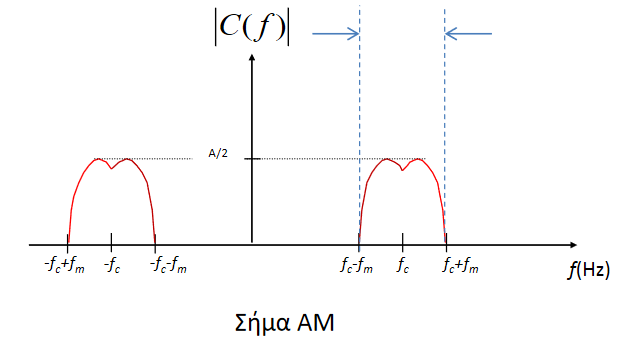
\includegraphics[scale=0.8]{papadop_1.png}
\end{center}
Λόγω της συνάρτησης Bessel, το σήμα σε διαμόρφωση φάσης (PM) θα μοιάζει με το παρακάτω γράφημα, ανάλογα με το $β$ που θα έχει:
\begin{center}
    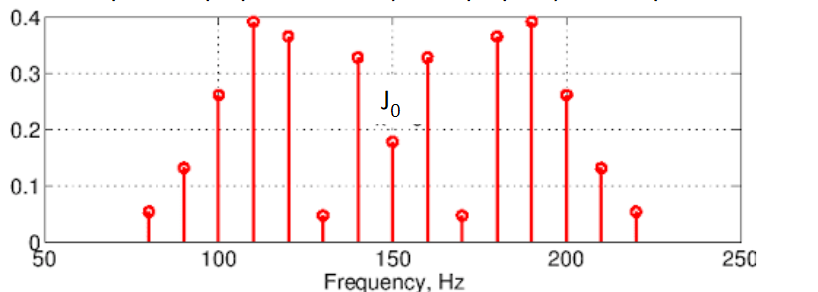
\includegraphics[scale=0.6]{papado3.png}
\end{center}
Οπότε το σήμα QAM, στο πεδίο της συχνότητας, θα μοιάζει με: 
\begin{center}
    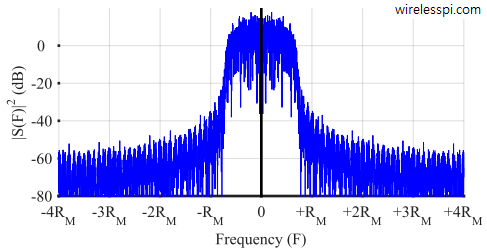
\includegraphics[scale=1]{papado4.png}
\end{center}
Τέλος, ας δούμε ένα 64-QAM χωρίς θόρυβο σε σύγκριση με ένα 64-QAM με θόρυβο:
\begin{center}
    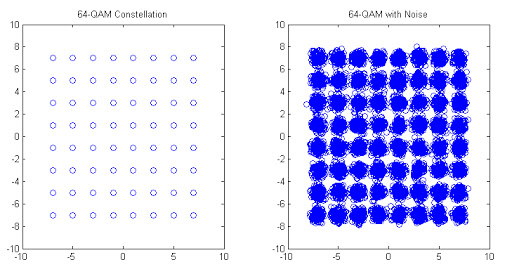
\includegraphics[scale=0.6]{noise_aaaaa.jpg}
\end{center}
\section{Βιβλιογραφία}
\small
[1] Stallings W. - Beard C., Ασύρματες Επικοινωνίες, Δίκτυα και Συστήματα, 2016\\[0pt]
[2] Louis E. Frenzel Jr, Electronics Explained (Second Edition), 2018\\[0pt]
[3] Hen-Geul Υeh, Victor Ramirez, Implementation and Performance of a M-ary PSK and QAM-OFDM System in a TMS320VC5416 Digital Signal Processor\\[0pt]
[4] IEEE Standard 802.11ac-2013\\[0pt]
[5] Vasilios C. Ilioudis, Wireless Sensors and Systems (Slides), 2021\\[0pt]
[6] Φωτεινή Παπαδοπούλου, Σήματα Πληρ. και Επικοινωνία (Σημειώσεις), 2020
\end{document}
